\chapter{Grundlagen und Begriffsbildung}\label{Kapitel 2}

Es gibt zahlreiche Benchmarks, die bereits an den RPi angepasst und auf diesem ausgef"uhrt wurden. Dabei steht oft die Performance verschiedener Betriebssysteme (z.B. Fedora vs. Debian) oder einzelner Hardware-Komponen\-ten im Vordergrund. Zu diesem Zweck werden haupts"achlich Linux-spezifische Benchmarks verwendet wie Sysbench CPU Benchmark (CPU), PyBench (Python-Implementierung), Apache Benchmark (Webserver), Open\-SSL (CPU) oder ioquake3 (GPU). 

Bei n"aherer Betrachtung erscheint es schwierig, sich einen "Uberblick "uber die existierenden Benchmarks zu verschaffen. Vieles, was von den Anwendern als "`Benchmark"' bezeichnet wird, stellt sich als selbst geschriebene Routine heraus, mit der z.B. die Performance der Grafikkarte getestet werden soll. Auf solche Routinen darf sich die Untersuchung nicht st"utzen. Im Folgenden wird daher auf grundlegende Begriffe der Untersuchung eingegangen. Anschlie\ss end werden die verwendeten Benchmarks (vgl. \ref{Benchmarks}) und ihre Anpassung an den RPi erl"autert (vgl. \ref{Aufbau}). 

\section{Definition: \textit{Benchmarking}}\label{Benchmarking}

Unter \textit{Benchmarking} oder "`Ma\ss st"abe vergleichen"' versteht man im Allgemeinen die vergleichende Analyse von Ergebnissen oder Prozessen mit einem festgelegten Bezugswert oder Vergleichsprozess. \textit{Computer-Benchmarks}, die hier von Bedeutung sind, dienen dem Vergleich der Rechenleistung von Computer-Systemen, wozu in der Regel Software verwendet wird:
\begin{quote}
\onehalfspacing
A simple method of measuring performance is by means of a benchmark program. [\dots] The intention is that by running it upon a new type of machine one may learn something of the performance the machine would have if it ran the original programs \cite{cur76}.
\end{quote}
Das \textit{Computer Lexikon 2012} kennt folgende Definition: 
\begin{quote}
\onehalfspacing
Mit einem Benchmark-Programm werden Hardwarekomponenten meist auf Geschwindigkeit getestet, wie z.B. die CPU, das Mainboard, die Festplatte (Schreib-Lese-Geschwindigkeit), die Grafikkarte (Frames/s) usw. Verschiedene Benchmark-Programme liefern oft unterschiedliche Ergebnisse, so dass ein direkter Vergleich zwischen den erreichten Werten kaum aussagekr"aftig ist \cite{pre11}. 
\end{quote}
Hieran wird deutlich, dass die Aussagekraft von Benchmarks eng mit der jeweiligen Testumgebung und der Zielsetzung des Benchmarks zusammenh"angt. Zwei Benchmarks, die die CPU-Performance evaluieren, liefern m"oglicherweise unterschiedliche Ergebnisse, weil unterschiedliche Parameter oder sogar Messgr"o\ss en zu Grunde liegen. Das ist insbesondere bei der Auswahl der Implementierungen und Gestaltung der Testumgebung zu ber"ucksichtigen (vgl. Kap. \ref{RPi-Spezi}, \ref{Bramble-Spezi} und \ref{Aufbau}). 

In dieser Arbeit soll die Leistung von Hardware-Komponenten eines oder mehrerer parallel arbeitender Rechenkerne mit standardisierten Verfahren ermittelt werden. Rechenberg bezeichnet "`\textit{Analyse}, \textit{Auswahl} und \textit{Konfiguration} von Gesamtsystemen aus Hardware und Software \cite{rec06}"' als eine Hauptaufgabe der Leistungsbewertung: 
\begin{quote}
\onehalfspacing
[F]"ur diese Aufgaben, die die etwa im Zuge einer Rechnerbeschaffung anfallen, wurde in Form von standardisierten Me\ss programmen und -methoden (\textit{benchmarking}) eine solide Basis geschaffen \cite{rec06}. 
\end{quote} 
Daher wird hier hier mit \textit{Benchmarking} das \textbf{\textit{Standardisieren von Arbeit}} bezeichnet.

% Def. Performance = Rechenleistung 
\section{Definition: \textit{Performance}}\label{Performance}

Die physikalische Gr"o\ss e \textit{Leistung} ist als \textit{Energie pro Zeit} definiert. In der Informatik wird der Begriff meist abweichend als Rechenleistung verwendet, d.h. das Zeitverhalten von Programmen und Ger"aten oder die Leistungsf"ahigkeit eines Computersystems. Eine Abgrenzung erscheint jedoch schwierig: 
\begin{quote}
\onehalfspacing
The performance of a computer is a complicated issue, a function of many interrelated quantities. These quantities include the application, the algorithm, the size of a problem, the high-level language, the implementation, the human level of effort used to optimize the program, the compiler's ability to optimize, the age of the compiler, the operating system, the architecture of the computer and the hardware characteristics \cite{don03}.
\end{quote}
Das \textit{Informatik-Handbuch} liefert folgende Aspekte:
\begin{quote} 
\onehalfspacing
Quantitative Leistungsanalysen (\textit{performance analyses}) ermitteln Leistungskenngr"o\ss en von Rechenanlagen. [\dots] Leistungsbewertung kann sich auf Teilschaltungen, Komponenten (wie Prozessor, Speichersystem oder periphere Ger"ate), gesamte Rechnerverb"unde beziehen \cite{rec06}.
\end{quote}
In dieser Arbeit soll die Performance eines RPis und eines RPi-Clusters bei der Ausf"uhrung von Benchmark-Programmen ermittelt werden. Curnow erl"autert in Bezug auf Whetstone: 
\begin{quote}
\onehalfspacing
We are not claiming [to reflect] the overall performance of a given system. On the contrary, we believe that no single number ever can. It does, however, reflect the performance of a dedicated machine for solving a dense system of linear equations \cite{cur76}.
\end{quote}
Mit \textit{Performance} wird daher hier die \textbf{\textit{Rechenleistung}} in diesem abgegrenzten Sinn bezeichnet, d.h. die Datenverarbeitungsgeschwindigkeit eines spezifischen Systems, nicht dessen Leistung im physikalischen Sinn. 

% Def.: Leistung = Time to Completion (lt. Christian, aber m.E. falsch - daher ersetzt durch Energieverbrauch)
%\section{Definition: \textit{Leistung}}\label{Leistung}
%
%Die physikalische Gr"o\ss e \textit{Leistung} ist als \textit{Energie pro Zeit} definiert. In der Informatik wird der Begriff meist abweichend verwendet: Laut Rechenberg sind wichtige Aspekte bei der Leistungsbewertung eines Rechnersystems das zu untersuchende System, die Arbeitslast und die Methode zur Leistungsermittlung (vgl. \cite{rec06}), au\ss erdem 
%\begin{quote}
%\onehalfspacing
%[...] die \textit{Leistungskenngr"o\ss en} oder \textit{-ma\ss zahlen} (\textit{performance metrics}), die f"ur das vorliegende Rechnersystem und die Ziele der Leistungsanalyse relevant sind \cite{rec06}. 
%\end{quote}
%Die hier verwendete Definition greift den ersten Aspekt auf: Mit \textit{Leistung} ist die \textbf{\textit{Time to completion}} gemeint, d.h. die Zeit, die ein Prozess oder ein Programm(teil) bis zum erfolgreichen Abschluss ben"otigt. Bei Rechenberg wird dies als "`Programmlaufzeit"' \cite{rec06} bezeichnet\footnote{Andere Klassen von Kenngr"o\ss en, die neben der Zeit zur Leistungsbewertung herangezogen werden, sind \textit{Durchsatz} und \textit{Auslastung}. Abweichende zeitliche Kenngr"o\ss en sind z.B. \textit{Bedienzeit (Service time)} oder \textit{TTR (Time to Response)} (vgl. \cite{rec06}).}. 

% Energieverbrauch = Exergieverbrauch/Entropieerzeugung in Watt
\section{Definition: \textit{Energieverbrauch}}\label{Energieverbrauch}

Obwohl der Begriff \textit{Energieverbrauch} (engl. \textit{energy consumption} oder \textit{power consumption}) weit verbreitet ist (vgl. z.B. \cite{fic13} und \cite{buh08}), stimmt er nicht mit der physikalischen Definition "uberein: Nach dem Energieerhaltungssatz bleibt die Gesamtenergie in einem geschlossenen System konstant. Dennoch wird der Begriff auch in der Informatik h"aufig verwendet, um die Leistungsf"ahigkeit eines Rechners oder Rechensystems in Abh"angigkeit von der Energieaufnahme zu charakterisieren:
\begin{quote}
\onehalfspacing
Vom physikalischen Standpunkt aus betrachtet, ist der Ausdruck "`Energieverbrauch"' falsch. Energie kann nicht verbraucht oder erzeugt, sondern nur umgewandelt werden. Trotzdem hat sich dieser Bergriff eingeb"urgert [\dots]. Bei elektronischen Systemen wird elektrische Energie verwendet, um Rechenleistung in einer bestimmten Zeitspanne zu generieren, physikalisch gesehen wird die elektrische Energie jedoch zu nahezu hundert Prozent in W"armeenergie umgewandelt \cite{lan13}. 
\end{quote}
In dieser Arbeit liegt ein Schwerpunkt der Leistungsbewertung auf der Energieaufnahme eines RPi-Clusters bei der Ausf"uhrung von Benchmark-Programmen. Mit \textit{Energieverbrauch} ist hier der Exergieverbrauch bzw. die Entropieerzeugung in Watt im physikalischen Sinn gemeint.     

\section{Benchmarks}\label{Benchmarks}

Aus der F"ulle an existierenden Benchmarks eine Auswahl zu treffen erweist sich als trickreich. M"ogliche Kriterien f"ur die Auswahl nennt Weicker: 
\begin{quote}
\onehalfspacing
The [\dots] best benchmark (1) is written in a high-level language, making it portable across different machines, (2) is representative for some kind of programming style (for example, systems programming, numerical programming, or commercial programming), (3) can be measured easily, and (4) has wide distribution \cite{wei90}. 
\end{quote}
Der Benchmark muss zudem "uberhaupt auf das gew"ahlte System anwendbar sein, d.h. das System muss dessen Spezifikationen erf"ullen bzw. es muss eine geeignete Implementierung vorliegen. Aus diesem Grund musste z.B. SHOC ausscheiden. SHOC ist nicht lauff"ahig auf dem RPi, da Open CL nicht unterst"utzt wird. 

F"ur die Untersuchung wurden drei etablierte HPC-Benchmarks vorgegeben, die sowohl auf Cluster-Architekturen als auch Einzelrechnern zur Anwendung kommen: Linpack, Whetstone und STREAM. Sie werden im Folgenden vorgestellt. 

\subsection{Linpack}\label{Linpack}

Grunds"atzlich muss zwischen der Linpack-Library und dem Linpack-Benchmark unterschieden werden: Erstere ist eine numerische Programmbibliothek zum L"osen von linearen Gleichungssystemen und galt darin lange Zeit als Standard. Der Linpack-Benchmark basiert auf zwei ihrer Routinen: 
\begin{quote}
\onehalfspacing
Linpack was designed out of a real, purposeful program that is now used as a benchmark \cite{wei90}. 
\end{quote}
Er wurde haupts"achlich von Jack Dongarra entwickelt und wird seit den 1970er Jahren zur Klassifizierung von Rechnern verwendet: 
\begin{quote}
\onehalfspacing
Over the years additional performance data was added [\dots] and today the collection includes over 1300 different computer systems \cite{don03}.
\end{quote}
Seit 1993 werden die leistungsf"ahigsten Supercomputer der Welt durch die Top500-Rankings ermittelt. Hierzu dient die Variante HPLinpack, auch $N\times N$ Linpack oder High Parallel Computing genannt:  
\begin{quote}
\onehalfspacing
Over recent years, the LINPACK Benchmark has evolved from a simple listing for one matrix problem to an expanded benchmark describing the performance at three levels of problem size on several hundred computers. The benchmark today is used by scientists worldwide to evaluate computer performance, particularly for innovative advanced-architecture machines \cite{don03}. 
\end{quote}
Dort findet sich auch eine vertiefte Darstellung des Linpack-Benchmarks. Der Quellcode findet sich unter \url{http://www.netlib.org/benchmark/1000d}.
% LU Factorization: 
%Will man das Lösen eines quadratischen eindeutig lösbaren Gleichungssystems Ax=b als Computerprogramm umsetzen, bietet es sich an, den Gaußalgorithmus als LR-Zerlegung (auch LU-Zerlegung oder Dreieckszerlegung genannt) zu interpretieren. Dies ist eine Zerlegung der regulären Matrix A in das Produkt einer linken unteren Dreiecksmatrix L (links, bzw. engl. „lower“) und einer rechten oberen Dreiecksmatrix R (rechts, auch mit U bezeichnet, von engl. „upper“)

% BLAS: Basic Linear Algebra Subroutines

\subsubsection{Funktionsweise}\label{Funktionsweise Linpack}

Linpack dient der Ermittlung der CPU-Leistung. Dazu werden Flie\ss punkt-Operationen auf einer Matrix durchgef"uhrt, die intern in eine lineare Darstellung umgewandelt wird. Das Ergebnis wird als \textit{Performance} in FLOPs ("`Floating Point Operations Per second"') ermittelt. Der Anteil der Nicht-Flie\ss punkt-Operationen wie Berechnungen auf Integer-Werten werden bei der Auswertung entweder vernachl"assigt oder in die Flie\ss punkt-Operationen integriert (vgl. \cite{wei90}). Die Linpack-Varianten Linpack 100, Linpack 1000 und HPLinpack verwenden Matrizen der Gr"o\ss e 100 $\times$ 100, 1000 $\times$ 1000 bzw. $n\times n$, d.h. eine Matrix variabler Gr"o\ss e, zur Berechnung. HPLinpack liefert Messergebnisse f"ur $R_{max}$ ("`Performance for the largest problem"'), $N_{max}$ ("`Size of the largest problem run"'), $N_{1/2}$ ("'Size where half the $R_{max}$ execution rate is achieved"') und $R_{peak}$ ("`Theoretical peak performance"') in \textit{FLOPs}. Entscheidend f"ur die Positionierung in der Top500-Liste ist dabei der $R_{max}$-Wert. Dabei erreicht der derzeit leistungsf"ahigste Supercomputer, \textit{Tianhe-2 (Milky\-Way-2)}, 33862.7 TFLOPS. \textit{SuperMUC}, der zuletzt auf Platz 10 der Top500 gerankt wurde, erzielte 2897.0 TFLOPS.

Beim Vergleich der Ergebnisse von Linpack ist die Matrixgr"o\ss e von Bedeutung, da ihre Ab"anderung bei unterschiedlichen Rechnerarchitekturen zu geringerer Datenlokalit"at und damit zu starken Abweichungen der Ergebnisse f"uhren kann (vgl. \cite{wei90}). In der Regel werden daher die oben genannten Matrixgr"o\ss en verwendet, obwohl der Quellcode eine "Anderung zul"asst. 

\subsubsection{Linpack auf dem Raspberry Pi}\label{Linpack RPi}

Bereits kurz nach Verkaufsstart des RPi wurden Implementierungen von Linpack f"ur den RPi bereit gestellt und Ergebnisse von Testl"aufen im Internet ver"offentlicht. Die hier verwendete Implementierung in C f"ur den RPi-Einzelrechner findet sich unter \url{http://www.roylongbottom.org.uk/Raspberry_Pi_Benchmarks.zip}. Somit liegen bereits Vergleichswerte f"ur einen RPi-Einzelrechner vor. Auch Implementierungen von Linpack f"ur verteilte Systeme unabh"angig von den Top500-Rankings sind im Umlauf (vgl. \url{http://www.netlib.org/benchmark/hpl}).

\subsection{Whetstone}\label{Whetstone}

Auch Whetstone ist als Benchmark im HPC-Bereich und zur Klassifizierung von Einzelrechnern seit vielen Jahren etabliert:
\begin{quote}
\onehalfspacing
[T]he most common 'stone age' benchmarks (CPU/memory/compiler benchmarks only) [are] in particular the Whetstone, Dhrystone, and Linpack benchmarks. These are the benchmarks whose results are most often cited in manufacturers' publications and in the trade press \cite{wei90}.
\end{quote}
Er wurde 1976 von Roy Longbottom u.A. entwickelt und gilt als erstes Programm, das jemals explizit f"ur das Benchmarking industrieller Standards designt wurde (vgl. \cite{wei90}). Wie Linpack misst er die CPU-Leistung. 

\subsubsection{Funktionsweise}\label{Funktionsweise Whetstone}

Die Funktionsweise von Whetstone "ahnelt Linpack. Allerdings werden nicht nur Flie\ss komma-Berechnungen ausgef"uhrt, sondern auch mathematische Funktionen, Integer-Arithmetik, bedingte Anweisungen etc. kommen zur Anwendung, da die urspr"ungliche Programmversion nicht komplex genug war, um ein durchschnittliches FORTRAN-Programm zu simulieren: Gegen"uber der urspr"unglichen Implementierung in ALGOL 60 war ein damals g"angiger FORTRAN-Compiler in der Lage, Zwischenergebnisse in schnellen Registern abzuspeichern und darauf zur"uckzugreifen. So fiel die gemessene CPU-Leistung deutlich h"oher aus als erwartet (vgl. \cite{cur76}). 

Die einzelnen Teile werden als Module bezeichnet und sind jeweils in eine For-Schleife eingebettet, die viele Male  hintereinander ausgef"uhrt wird. Ein Rahmenprogramm steuert Aufruf der Module und Ausgabe der Ergebnisse. Auch die Ausgabe ist Teil des Benchmarks, allerdings bemerkt Curnow hierzu: 
\begin{quote}
\onehalfspacing
This output is only required to ensure that the calculations are logically necessary; it is not intended to represent the output from a typical program \cite{cur76}. 
\end{quote}
Die Ergebnisse wurden zun"achst in \textit{Whetstone Instructions per Second} gemessen, heutige Implementierungen liefern Ergebnisse in MFLOPs. Eine detaillierte Darstellung der Entwicklung und Implementierung von Whetstone findet sich bei \cite{cur76}, ebenso der urspr"ungliche Quellcode in ALGOL 60. 
% Least-squares: 
%Die Methode der kleinsten Quadrate ist das mathematische Standardverfahren zur Ausgleichungsrechnung. Dabei wird zu einer Datenpunktwolke eine Kurve gesucht, die möglichst nahe an den Datenpunkten verläuft.

\subsubsection{Whetstone auf dem Raspberry Pi}\label{Whetstone RPi}

Whetstone erschien wie f"ur den RPi gemacht, da er sich als Standard f"ur Mini-Computer etabliert hat: Der Benchmark war in den 70er Jahren f"ur Maschinen mit deutlich geringerer Rechenleistung als heute entwickelt worden. Bereits damals gingen die Entwickler von notwendigen Anpassungen f"ur neue Speicherhierarchien aus: 
\begin{quote}
\onehalfspacing
When more is known about the characteristics of programs running on these multi-level store machines it may be possible to produce a typical program for particular types of machine. [\dots] Despite these limitations the program described should be of some value, particularly in relation to smaller machines \cite{cur76}. 
\end{quote}
Er wurde vom Entwickler selbst f"ur den RPi angepasst und und auf diesem getestet (vgl. \url{http://www.roylongbottom.org.uk/Raspberry\%20Pi\%20Benchmarks.htm.}. Auch hier liegen also Vergleichswerte f"ur einen RPi-Einzelrechner vor. 

Wie f"ur die meisten etablierten HPC-Benchmarks existieren Implementierungen in h"oheren Programmiersprachen wie C, C++, Fortran und Java (vgl. \url{http://freespace.virgin.net/roy.longbottom}). Auch hier wird auf eine Implementierung in C f"ur den RPi-Einzelrechner zur"uckgegriffen. Der Quellcode findet sich unter \url{http://www.roylongbottom.org.uk/}\newline \url{Raspberry_Pi_Benchmarks.zip}. Ob eine lauff"ahige Implementierung f"ur die Cluster-Archi\-tektur existiert, wird sich zeigen m"ussen. 

\subsection{STREAM}\label{STREAM}

Mit zunehmender Rechenleistung der Prozessoren und der Zunahme an Prozessorkernen innerhalb eines Rechnersystems zeigte sich, dass es nicht ausreicht, die Leistungsf"ahigkeit lediglich an Hand der CPU-Leistung zu bewerten. Zudem l"asst sich eine Tendenz beobachten, dass Rechnersysteme gezielt f"ur die Ausf"uhrung bestimmter Benchmarks wie HPLinpack optimiert werden, um z.B. in Rankings bessere Wertungen zu erreichen. 

STREAM wurde mit dem Ziel entwickelt, das Verh"altnis von CPU-Leistung zu Speichergeschwindigkeit in die Bewertung einzubeziehen. Mittlerweile ist STREAM auch Bestandteil der HPCChallenge Benchmark-Suite, ein Rahmenwerk mit der Zielsetzung, Anforderungen aus der Anwendungspraxis in die Bewertung von HPC-Rechnersystemen einflie\ss en zu lassen (vgl. \cite{lus05}).

%Die Zunahme an Prozessorleistung f"uhrt jedoch nicht notwendigerweise zu einer Verbesserung der Gesamtleistung eines Systems. Gerade bei Supercomputern besteht ein potenzieller Flaschenhals oft nicht in der mangelnden Leistung der einzelnen Rechnerkerne, sondern in der Performance von I/O-Zugriffen auf den nicht fl"uchtigen Speicher\footnote{Vgl. \cite{mcc95}.}. Zudem besteht zwischen der Performance, die mit Benchmarks wie HPLinpack ermittelt wird, und den tats"achlichen Anforderungen heutiger Programme oft kein proportionaler Zusammenhang. D.h. Maschinen, die sehr gute Werte bei Linpack oder Whetstone erzielen, k"onnen diese unter der Workload konkreter Anwendungen unter Umst"anden oftmals nicht halten. Andererseits k"onnen deutlich leistungsschw"achere Rechnersysteme bei bestimmten Anwendungen "ahnlich gute Werte erreichen wie weitaus besser gerankte Maschinen aus den Top500, wenn diese gr"o\ss tenteils auf gecachten Daten arbeitet und wenige Zugriffe auf den nicht fl"uchtigen Speicher erfordert\footnote{Vgl. ebd.. Dieses Ph"anomen zeigte sich im HPC-Bereich seit ca. 1990 und wurde von Eugene Brooks bei der Supercomputing-Konferenz 1989 als "`attack of the killer micros"' bezeichnet (vgl. ebd.).}. 

\subsubsection{Funktionsweise}\label{Funktionsweise STREAM}

STREAM ist ein synthetischer Benchmark und basiert auf einem Programm aus der wissenschaftlichen Praxis von John McCalpin, das die dauerhafte Speicher-Bandbreite (engl. "`sustainable memory bandwidth"' \cite{mcc95}) f"ur angrenzende Speicherzugriffe langer Vektoren (engl. "`sustainable memory bandwidth for contiguous, long-vector memory accesses"'\cite{mcc95}) ermittelt. Die Vektoren m"ussen lang genug sein, dass sie nicht im Prozessor-Cache vorgehalten, sondern aus dem nicht fl"uchtigen Speicher geladen werden. STREAM ist somit Teil eines neuen Modells, das als Performance-Ma\ss zahl die Gesamtzeit $T_{total} = T_{cpu}$ (CPU-Performance) + $T_{memory}$ (Speicher-Performance, ermittelt durch STREAM) festlegt (vgl. \cite{mcc95} und \cite{mcc05}). 

STREAM durchl"auft bei seiner Ausf"uhrung vier Module (Copy, Scale, Add und Triad) und liefert f"ur jedes Modul die durchschnittliche, maximale und minimale Ausf"uhrungszeit sowie die Ausf"uhrungsrate. Jedes Modul wird mehrfach ausgef"uhrt, um verl"assliche Mittelwerte zu erhalten. Zwischen dem Programmcode der Module bestehen Abh"angigkeiten, um starke Optimierungen durch den Compiler zu verhindern (vgl. \cite{mcc05}). Quellcode und Ergebnisse f"ur STREAM auf verschiedenen Systemen finden sich unter \url{http://www.cs.virginia.edu/stream}.   

\subsubsection{STREAM auf dem Raspberry Pi}\label{STREAM RPi}

Auch f"ur STREAM wurden Ergebnisse auf einem RPi-Einzelrechner bereits ver"offentlicht (vgl. \url{http://www.cs.virginia.edu/stream/stream_mail/2012/0002.html}). Der auf dem RPi-Einzelrechner verwendete Quellcode findet sich unter \url{http://www.cs.virginia.edu/stream/FTP/Code/stream.c}. Die auf dem RPi-Cluster verwendete Implementierung findet sich unter \url{http://www.cs.virginia.edu/stream/FTP/Code/Versions/stream_mpi.f}.  

\section{Spezifikation des RPi Modell B}\label{RPi-Spezi}

Was dem Nutzer zuerst auff"allt, ist sicherlich die Gr"o\ss e des RPi. Er wird manchmal als "`Scheckkarten-Computer"' bezeichnet und "uberschreitet diese Ma\ss e mit 85.60 mm $\times$ 53.98 mm $\times$ 17 mm tats"achlich nur geringf"ugig. Auf dieser Platine sind alle Komponenten verbaut, die den RPi zu einem voll funktionsf"ahigen Rechner machen.

\subsection{System on a Chip, CPU, GPU und Arbeitsspeicher}\label{RPi-Hardware}

Der RPi ist mit einem Broadcom BCM2835 als System on a Chip ausgestattet. Es enth"alt CPU (ein ARM1176JZFS-Prozessor) und GPU (ein Broadcom VideoCore IV-Koprozessor, vgl. \cite{scrguide02}). Auff"allig ist, dass die CPU des RPi (ein ARM-Chip, wie er auch in Mobiltelefonen zur Anwendung kommt), relativ schwach ist im Vergleich zur GPU. Diese unterst"utzt Full HD-Aufl"osung und das Hardware-beschleunigte Rendern verschiedener Videoformate. Das Modell B verf"ugt "uber 512 MB SDRAM. Er kann nicht erweitert werden, doch die Aufteilung zwischen CPU und GPU ist variabel. Da der RPi kein BIOS hat, muss dazu die Datei \texttt{/boot/start.elf} manipuliert werden (vgl. \cite{pow12}).

\subsubsection{Schnittstellen}\label{RPi-Schnittstellen}

Der RPi verf"ugt "uber einen HDMI-Ausgang, einen Cinch-Ausgang ("`RCA Jack"') und einen analogen Tonausgang. Er hat zwei USB 2.0-Schnittstellen und eine RJ45-Buchse zum Anschluss einer 10/100 Base-T Ethernet-Schnittstelle. Ein Steckplatz ist f"ur eine SD-Karte vorgesehen, auf der der nicht fl"uchtige Speicher liegt. Die Stromversorgung erfolgt "uber einen Mini-USB-Eingang. Zum Betrieb werden 700 mA/5 V ben"otigt (vgl. \cite{pow12}). Der Vollst"andigkeit halber sei das Vorhandensein einer Allzweckeingabe/-ausgabe mit sechs Anschl"ussen und jeweils 26 Pins erw"ahnt. Dar"uber k"onnen, "ahnlich wie bei einem Arduino-Board, z.B. LEDs, Sensoren und Displays angesteuert werden. 

% RJ45: Vollbeschaltetes 8P8C ohne Widerstände; eigentlich RJ-48, RJ-49 oder RJ-61
% 10/100 Base-T: Buchse für Ethernet-Schnittstelle mit Datenrate 10/100 Mbps, Baseband u. Twisted-Pair-Kabel

\subsection{Betriebssystem}\label{RPi-OS}

F"ur den RPi existieren mehrere Varianten bzw. Derivate verbreiteter Betriebssysteme. Am verbreitetsten sind Linux/Unix-basierte Systeme wie FreeBSD und NetBSD (BSD-Varianten), Raspbian (Debian-Variante), Pidora (Fedora-Variante) oder eine Variante von Arch Linux (vgl. \cite{pow12}). Daneben gibt es Implementierungen von RISC OS und Plan 9. Als Betriebssytem f"ur den RPi-Einzelrechner wurde Raspbian gew"ahlt, die offizielle Distribution der Raspberry Pi Foundation (vgl. \url{http://www.raspberrypi.org/faqs}). Das hier verwendete Abbild findet sich unter \url{http://downloads.raspberrypi.org/raspbian_latest}. 

\section{Raspberry Pi-Cluster als Testumfeld}\label{Bramble-Spezi}

Seit einiger Zeit l"asst sich die Tendenz beobachten, eine gr"o\ss ere Anzahl von Raspberry Pis zu einem Cluster zu koppeln (weitere Projekte werden in \cite{cox13}, \cite{kie01}, \cite{bal12} und \cite{ou13} dargestellt). Die hier verwendete Architektur wird im Folgenden kurz vorgestellt. Eine detaillierte Darstellung liefert \cite{kli13}. 

\subsection{Physischer Aufbau}\label{Bramble-Hardware}

Der RPi-Cluster besteht aus 20 RPi Modell B-Einzelrechnern ((1), DNS-Namen \texttt{pi01} -- \texttt{pi20}). Sie sind jeweils "uber ein Ethernet-Kabel (2) mit einem 24 Port Gigabit-Switch (3) verbunden, der an einen zentralen x86-Server (DNS-Name \texttt{careme}) angeschlossen ist. 

Er besteht aus einem Mini-ITX-Mainboard (4) und % TODO: wie viele? 
Festplatten mit einem Software-RAID Level 5-System f"ur den Netzwerkzugriff und einem RAID Level 1-System f"ur das Betriebssystem (5).  

Die Stromversorgung erfolgt "uber ein zentrales Netzteil (6). Daran sind zwei Verteiler (7) angeschlossen, an die jeweils 10 RPi-Einzelrechner "uber Mini-USB-Kabel (8) verbunden sind. 

Alle Komponenten befinden sich in einem Metallgeh"ause, in dessen Mitte drei K"uhlgebl"ase angebracht sind. 
%\begin{enumerate}
%	\item RPi-Einzelrechner
%	\item Ethernet-Kabel
%	\item 24 Port-Gigabit-Switch  
%	\item Mini-ITX-Mainboard
%	\item Festplatten (RAID Level 5 als I/O-Shield, RAID Level 1 f"ur Betriebssystem)
%	\item Netzteil
%	\item Verteiler 
%	\item Mini-USB-Kabel 
%	\item K"uhlgebl"ase
%\end{enumerate}
\begin{figure}[htb]
	\centering
	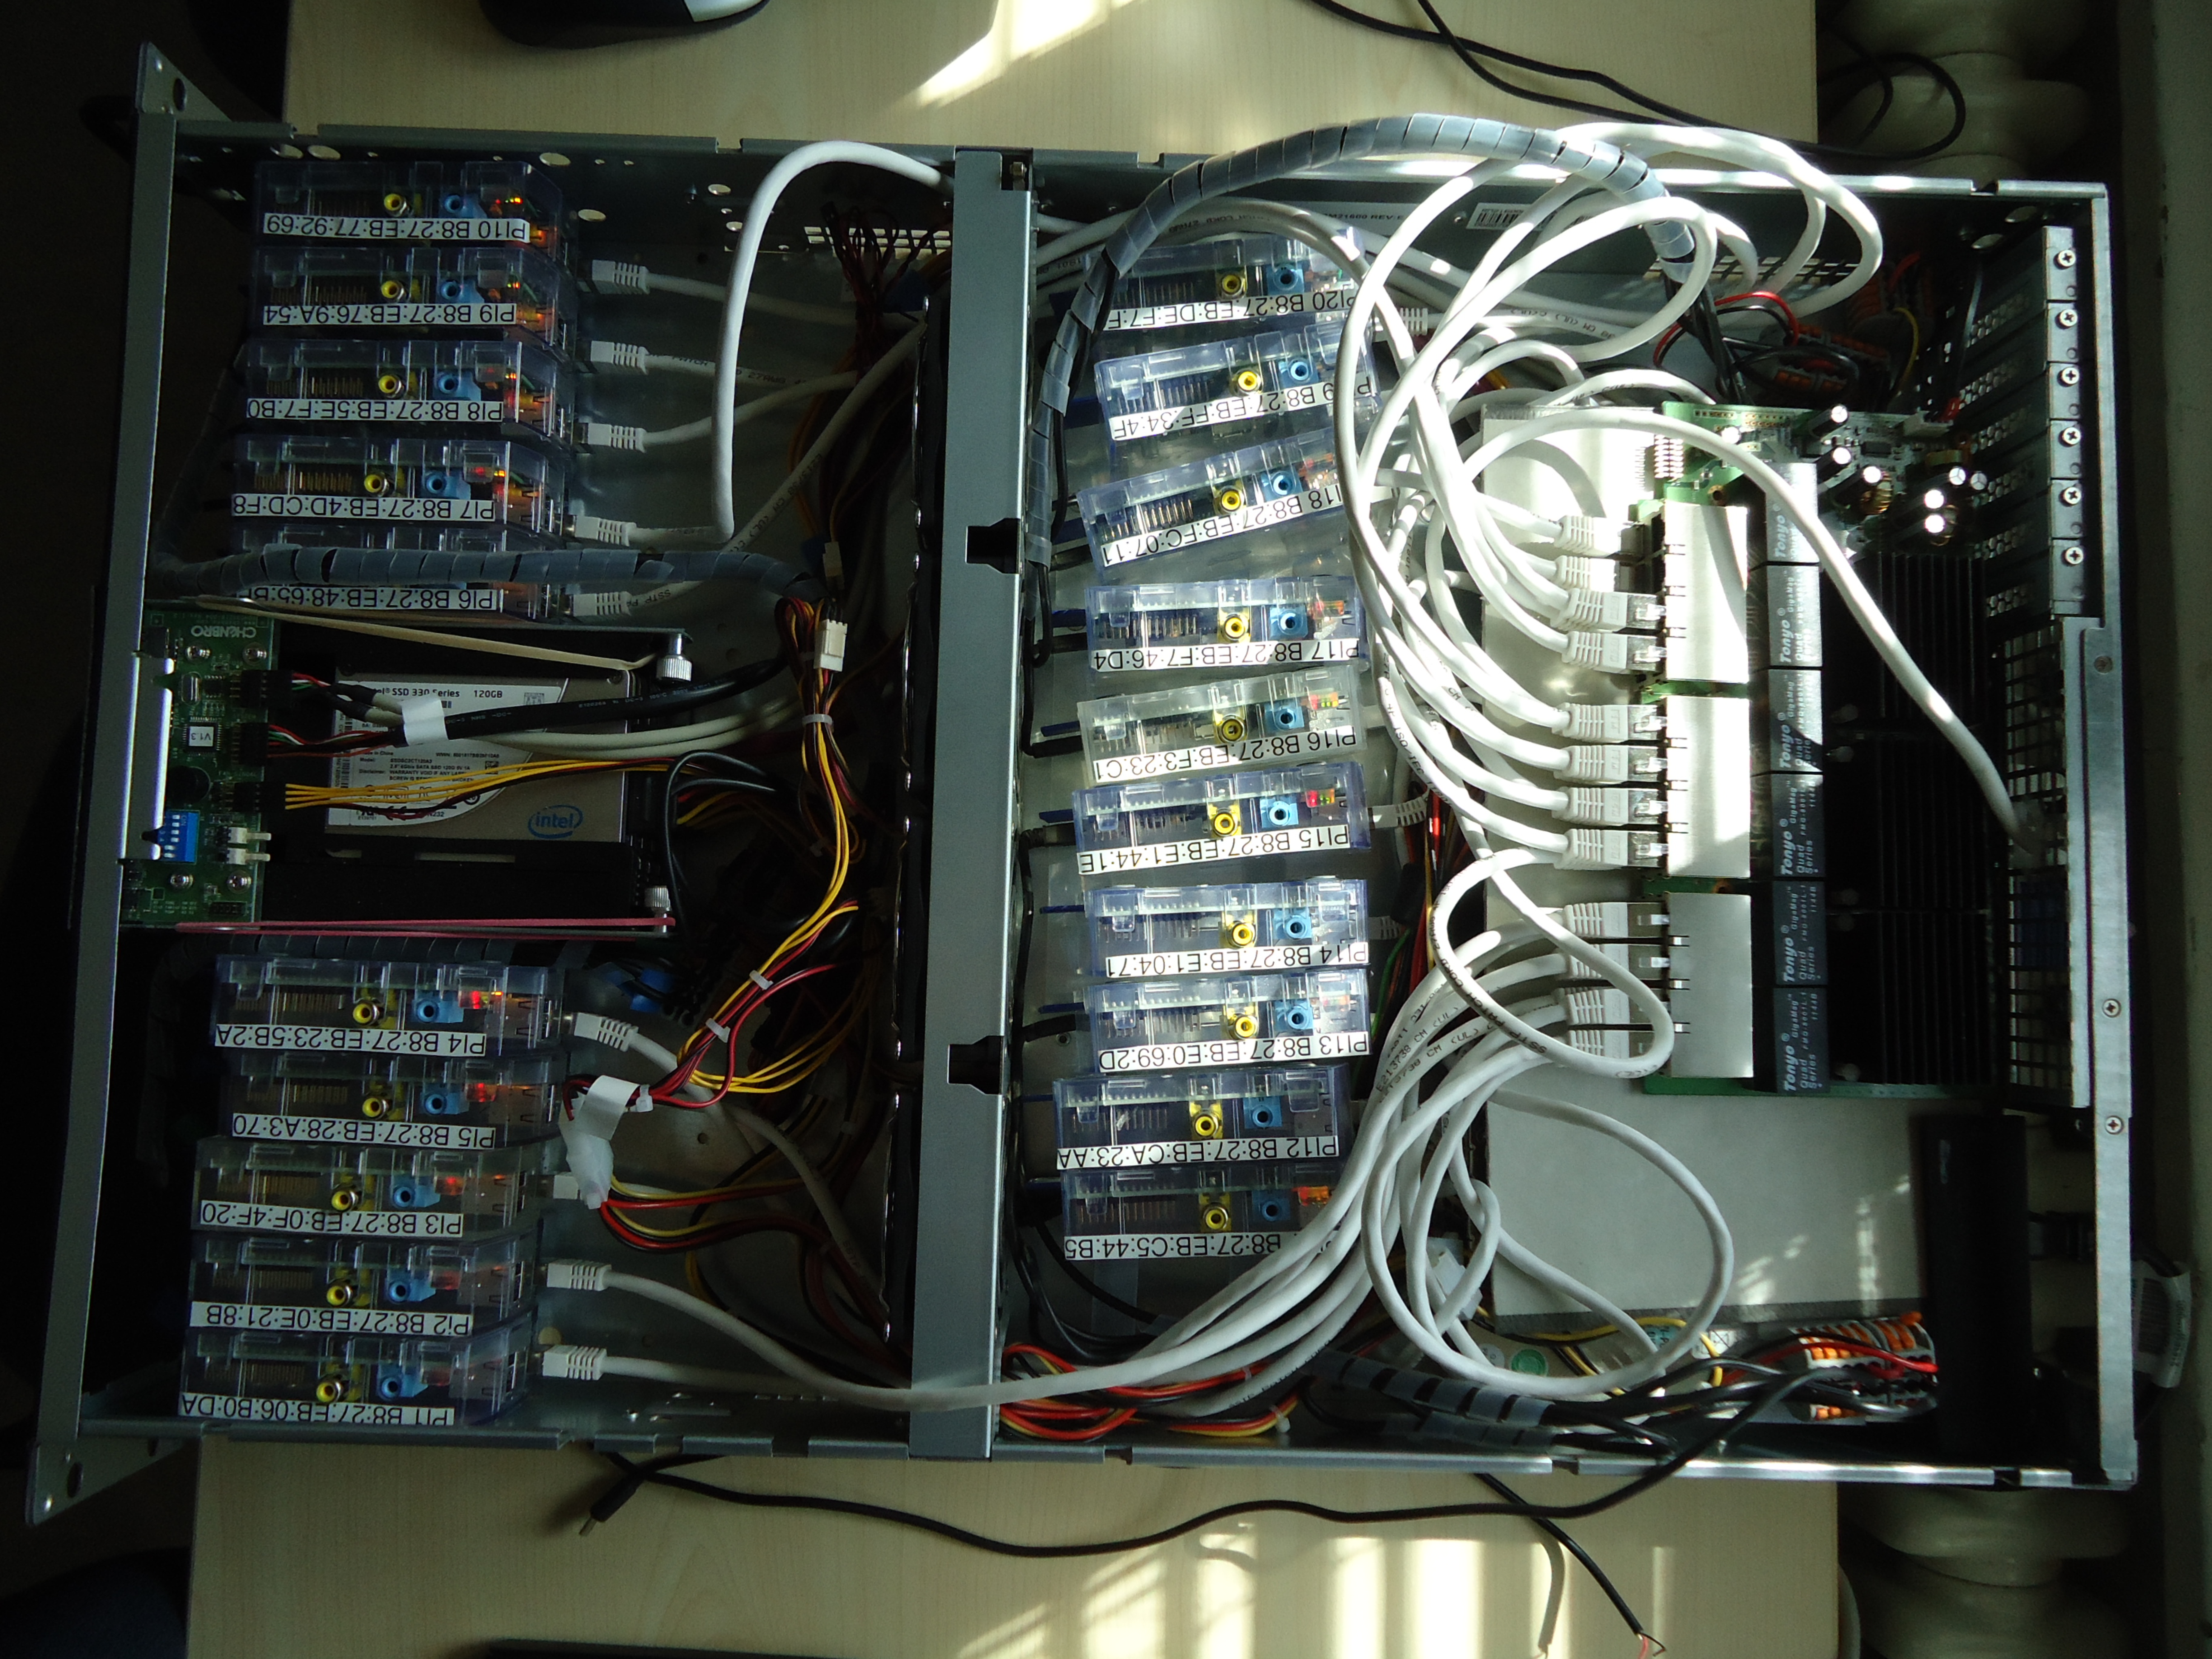
\includegraphics[width=0.7\textwidth]{bramble.pdf}\\ 
	\caption{Schematischer Aufbau des hier verwendeten Bramble.}\label{fig:Bramble}
\end{figure}
% NIC = Network Interface Card 
Ein solches System relativ kosteng"unstiger Rechner mit einem BSD- oder Linux-Betriebs\-system, die "uber IP kommunizieren, wird im Allgemeinen als \textit{Beowulf} bezeichnet (vgl. \cite{kie01}). Es kann der Simulation eines Supercomputers dienen. Im Zusammenhang mit RPis wird auch der Begriff \textit{Bramble} "ublich, der im Folgenden verwendet wird (vgl. \url{www.raspberrypi.org/archives/tag/bramble}). 
\subsection{Betriebssystem und Dateisystem}\label{Bramble-Architektur} 

Auf den RPi-Nodes l"auft das o.g. Betriebssytem Raspbian, auf \texttt{careme} eine Standard-Debian-Version. Ein Charakteristikum eines Beowulf-Clusters bzw. Bramble ist, dass es kein Shared Memory-Interface und keine Cache-Koh"arenz gibt. Somit stellt sich die Frage nach der Zeit- und Datensynchronisation der RPi-Knoten und des Servers sowie der M"oglichkeit eines gemeinsamen Speicherzugriffs. 

Grunds"atzlich werden zwei Dateisysteme auf dem Bramble eingesetzt: NFS ("`Network File System"') f"ur die root-Verzeichnisse der RPi-Knoten und ein Union-Dateisystem 
% NFS 
% Union Dateisystem
% Synchronisation 
% gemeinsames Verzeichnis 

%Um das Filesystem der einzelnen Nodes mit dem NFS des Servers zu synchronisieren, wurde hier eine Read-Only-Schicht f"ur die Slaves (Nodes) und eine Read-Write-Schicht f"ur den Master (Server) verwendet\footnote{Vgl. \cite{kli13}.}. Um trotzdem den gemeinsamen Zugriff von Server und RPi-Nodes auf ein Speichermedium zu erm"oglichen, wurde ein geshartes Verzeichnis \texttt{/srv} bzw. \texttt{/srv/nfs-share} eingerichtet. 

\subsection{Zugriff auf die Cluster-Komponenten}\label{Zugriff}

Welche M"oglichkeiten gibt es nun, verteilte Anwendungen auf dem Bramble auszuf"uhren bzw. "uberhaupt die einzelnen Komponenten anzusprechen? Der Zugriff auf den Bramble erfolgt aus dem internen Netz "uber IP und SSH. Die einzelnen RPi-Nodes werden von \texttt{careme} aus "uber SSH adressiert (private Adressen \texttt{10.0.0.2} bis \texttt{10.0.0.21}). Es gibt auf jedem RPi-Knoten den Raspbian-Standard-User \texttt{pi}, der hier nicht ver"andert wurde\footnote{Auf dem RPi-Einzelrechner wurden aus Sicherheitsgr"unden Username und Passwort f"ur den Standard-User ge"andert.}. Um z.B. auf das gesharte Verzeichnis \texttt{/srv} zuzugreifen, sind \texttt{root}-Berechtigungen erforderlich\footnote{Auf Schwierigkeiten dieser Einteilung und L"osungsans"atze wird in Kap. \ref{Bramble-Versuchsaufbau} eingegangen.}. 

Beim hier verwendeten Versuchsaufbau wurde auf \texttt{careme} mit eingeschr"ankten Rechten als User \texttt{rpi-user} gearbeitet, auf den einzelnen RPis als \texttt{root}. Das bedeutet, dass alle "Anderungen im gesharten Verzeichnis notwendigerweise von einem der RPi-Nodes aus vorgenommen werden m"ussen. Dazu wurde vorab RPi-Node \texttt{pi03} als Berechnungs-Node definiert, von dem aus alle Skripte ausgef"uhrt, Programme installiert werden etc.. Da die Skripte zur Ausf"uhrung der Benchmarks h"aufig das Herunterfahren einzelner RPi-Nodes vorsehen (vgl. Kap. \ref{Anhang}), wurden die Benchmarks grunds"atzlich auf maximal n=19 RPi-Nodes ausgef"uhrt (vgl. Kap. \ref{Kapitel 3}). Zur verteilten Berechnung von Anwendungen auf mehreren CPUs steht auf dem Bramble die MPI-Implementierung MPICH in der Version 3.0.4 zur Verf"ugung. Um die CPUs bzw. RPi-Nodes und die Anzahl der darauf auszuf"uhrenden Prozesse zu spezifizieren, muss ein entsprechendes Machinefile erstellt und im gesharten Verzeichnis abgelegt werden, das der Ausf"uhrung von MPICH mit \texttt{mpiexec} als Parameter "ubergeben wird (vgl. Kap. \ref{Kapitel 3}). 
\endinput 